\documentclass{ximera}

\newcommand{\RR}{\mathbb R}
\renewcommand{\d}{\,d}
\newcommand{\dd}[2][]{\frac{d #1}{d #2}}
\renewcommand{\l}{\ell}
\newcommand{\ddx}{\frac{d}{dx}}
\newcommand{\dfn}{\textbf}
\newcommand{\eval}[1]{\bigg[ #1 \bigg]}

\author{Jim Talamo}

\outcome{Define a series.}
\outcome{Recognize a geometric series.}
\outcome{Recognize a telescoping series.}
\outcome{Compute the sum of a geometric series.}
\outcome{Compute the sum of a telescoping series.}

\title[Dig-In:]{What is a series}

\begin{document}
\begin{abstract}
A series is an infinite sum of the terms of sequence.
\end{abstract}
\maketitle

In the previous sections, we've seen several examples of sequence.  If we have a sequence $\{a_n\}_{n=1}$, and represent it as an ordered list below: 

\[
a_1, a_2, a_3 , \ldots
\]

we can ask two important questions about it.

\begin{itemize}
\item[1.] Do the numbers in the list approach a finite value?
\item[2.] Can I sum all of the numbers in the list and obtain a finite result?
\end{itemize}

The first question is really whether the \emph{limit} $\lim_{n \to \infty} a_n$ exists and we studied several ways to determine this previously.  As it turns out, the second question is closely related to the first one.  We motivate this through an example.

\begin{example} Shading A Square

Suppose that we want to study the infinite sum below.

\[
\frac{1}{2} + \left(\frac{1}{2}\right)^2+ \left(\frac{1}{2}\right)^3+ \ldots
\]

A student, feeling quite clever, decides to illustrate the sum by drawing a square with side length one unit and shading it in a special way.  In order to understand the concepts here more fully, it is recommended that you draw and shade as you read.

\paragraph{Step 1:} Shade the left half of the square.  

\begin{image}[1in]
  \begin{tikzpicture}[scale=3,rounded corners=.5pt]      
    \tkzDefPoint(0,0){A1} 
    \tkzDefPoint(1,0){A2}
    \tkzDefPoint(1,1){A3}
    \tkzDefPoint(0,1){A4}
    \draw[penColor,very thick] (A1)--(A2)--(A3)--(A4)--cycle;

    \tkzDefPoint(0,0){B1} 
    \tkzDefPoint(.5,0){B2}
    \tkzDefPoint(.5,1){B3}
    \tkzDefPoint(0,1){B4}
    \draw[penColor,fill=fill2,very thick] (B1)--(B2)--(B3)--(B4)--cycle;
  \end{tikzpicture}

\end{image}
There are two quantities of which we can keep track now.
\begin{itemize}
\item Call the area shaded this step $A_1$.  Then, we have $A_1=\answer[given]{1/2}$.
\item Call and the total shaded area  of the square $S_1$.  Then, we have $S_1=\answer[given]{1/2}$.
\end{itemize}

\paragraph{Step 2:} Shade the bottom half of the unshaded region.  

\begin{image}[1in]
  \begin{tikzpicture}[scale=3,rounded corners=.5pt]      
    \tkzDefPoint(0,0){A1} 
    \tkzDefPoint(1,0){A2}
    \tkzDefPoint(1,1){A3}
    \tkzDefPoint(0,1){A4}
    \draw[penColor,very thick] (A1)--(A2)--(A3)--(A4)--cycle;

    \tkzDefPoint(0,0){B1} 
    \tkzDefPoint(.5,0){B2}
    \tkzDefPoint(.5,1){B3}
    \tkzDefPoint(0,1){B4}
    \draw[penColor,fill=fill1,very thick] (B1)--(B2)--(B3)--(B4)--cycle;
    
    \tkzDefPoint(.5,0){C1} 
    \tkzDefPoint(1,0){C2}
    \tkzDefPoint(1,.5){C3}
    \tkzDefPoint(.5,.5){C4}
    \draw[penColor,fill=fill2,very thick] (C1)--(C2)--(C3)--(C4)--cycle;
    
  \end{tikzpicture}
\end{image}

\begin{itemize}
\item Call the area shaded this step $A_2$.  Then, we have $A_2=\answer[given]{1/4}$.
\item Call and the total shaded area  of the square $S_2$.  Then, we have $S_2=\answer[given]{3/4}$.
\end{itemize}

Visually, notice that we can find $S_2$ by noting
$$(area ~ shaded ~ after ~ Step ~ 2) = (area ~ from ~ Step ~ 1) + (area ~ from ~ Step ~ 2)$$
and writing down the total shaded are of the square.

Analytically, we can write $S_2=A_1+A_2.$

\paragraph{Step 3:} Shade the left half of the unshaded region.  \begin{image}[1in]
  \begin{tikzpicture}[scale=3,rounded corners=.5pt]      
    \tkzDefPoint(0,0){A1} 
    \tkzDefPoint(1,0){A2}
    \tkzDefPoint(1,1){A3}
    \tkzDefPoint(0,1){A4}
    \draw[penColor,very thick] (A1)--(A2)--(A3)--(A4)--cycle;

    \tkzDefPoint(0,0){B1} 
    \tkzDefPoint(.5,0){B2}
    \tkzDefPoint(.5,1){B3}
    \tkzDefPoint(0,1){B4}
    \draw[penColor,fill=fill1,very thick] (B1)--(B2)--(B3)--(B4)--cycle;
    
    \tkzDefPoint(.5,0){C1} 
    \tkzDefPoint(1,0){C2}
    \tkzDefPoint(1,.5){C3}
    \tkzDefPoint(.5,.5){C4}
    \draw[penColor,fill=fill1,very thick] (C1)--(C2)--(C3)--(C4)--cycle;
    
    \tkzDefPoint(.5,.5){D1} 
    \tkzDefPoint(.75,.5){D2}
    \tkzDefPoint(.75,1){D3}
    \tkzDefPoint(.5,1){D4}
    \draw[penColor,fill=fill2,very thick] (D1)--(D2)--(D3)--(D4)--cycle;
    
  \end{tikzpicture}
\end{image}

\begin{itemize}
\item Call the area shaded this step $A_3$.  Then, we have $A_3=\answer[given]{1/8}$.
\item Call and the total shaded area  of the square $S_3$.  Then, we have $S_3=\answer[given]{7/8}$.
\end{itemize}

We can think of $S_3$ visually or analytically. 

%\begin{image}[1in]
%  \begin{tikzpicture}[scale=3,rounded corners=.5pt]      
%    \tkzDefPoint(0,1){A1} 
%    \tkzDefPoint(-.58,0){A2}
%    \tkzDefPoint(.58,0){A3}
%    \draw[penColor,very thick] (A1)--(A2)--(A3)--cycle;
%  \end{tikzpicture}
%\end{image}


%\begin{figure}[!htb]
%\minipage{0.32\textwidth}
%  \includegraphics[width=\linewidth]{SquareA1}
% \phantom{n}  \hspace{17mm} Step 1 
% 
%  \hspace{19mm}  $S_1 = A_1$
%  \endminipage\hfill
%\minipage{0.32\textwidth}
%  \includegraphics[width=\linewidth]{SquareA2}
%   \phantom{n}  \hspace{17mm} Step 2
% 
% \hspace{15mm}  $S_2=A_1+A_2$
%\endminipage\hfill
%\minipage{0.32\textwidth}%
%  \includegraphics[width=\linewidth]{SquareA4}
%   \phantom{n}  \hspace{17mm} Step 4
%   
%  \hspace{5mm}    $S_4=A_1+A_2+A_3+A_4$
%\endminipage
%
%\caption{\small The area $A_n$ shaded in the $n$-th step is shown in blue.  The total shaded area $s_n$ is the sum of the all of the areas shaded in each previous step as well as the current one.}
%\end{figure}

\vspace{3mm}

Hopefully, the pattern used to shade the square is becoming clear.  We can define the area  shaded during the $n$-th step to be $A_n$, and can observe that $A_n=(1/2)^n$.

We can also let $s_n$ denote the total shaded area after the $n$-th step.  Analytically, we have $S_n = A_1+A_2 + \ldots A_n$, or by using summation notation, we can write $\displaystyle S_n = \sum_{k=1}^n A_k$.

Looking at the pictures drawn so far, notice that the only unshaded area after the $n$-th step is a rectangle of area $A_n$, so we can write a formula for $s_n$.   

\[
S_n = \left<\textrm{area of the square}\right>-A_n = 1-\left(\frac{1}{2}\right)^n
\]

We can now evaluate the limit and find that $\lim_{n \to \infty} s_n =\answer[given]{1}$.

We also have another method of thinking about this limit; after we continue shading the square indefinitely, there will be no portion of it that has not been shaded.  Thus, the total shaded area should be $1$.

We would thus like to conclude that

\[
\frac{1}{2} + \left(\frac{1}{2}\right)^2+ \left(\frac{1}{2}\right)^3+ \ldots = \sum_{k=1}^{\infty} \left(\frac{1}{2}\right)^n =1.
\]
\end{example}

\section{Infinite series}
The above scenario can be modeled using sequences.  We have $\{A_n\}_{n=1}$ whose $n$-th term is given by the explicit formula $A_n=\left(\frac{1}{2}\right)^n$, and we represent the sequence by the ordered list below.

\[
\frac{1}{2},\left(\frac{1}{2}\right)^2,\left(\frac{1}{2}\right)^3,\ldots
\]
and we can interpret the series $$\frac{1}{2} + \left(\frac{1}{2}\right)^2+ \left(\frac{1}{2}\right)^3+ \ldots$$ as the attempt to add up all of the terms in the above sequence.  In order to determine if this can be done, we found a new sequence $\{S_n\}_{n=1}$ that was created from the original sequence.  It is represented by the list below.

\[
\frac{1}{2},\frac{3}{4},\frac{7}{8},\ldots
\]

Note that the \emph{limit} of this new sequence is exactly the \emph{sum} of all of the terms in the old sequence!  Let's formalize the ideas in the last example with a definition.

\begin{definition}
Let $\{a_n\}_{n=n_0}$ be a sequence.  Let $s_n = \sum_{k=k_0}^n a_k$; the sequence $\{s_n\}_{n=k_0}$ is the called the
  \dfn{sequence of partial sums} of $\{a_n\}$.  

\begin{enumerate}
\item The series $\sum_{k=k_0}^\infty a_k$ \dfn{converges} if and only if $\lim_{n\to\infty} s_n$ exists.  Furthermore, if $\lim_{n\to\infty} s_n =L$, we say the series $\sum_{k=k_0}^\infty a_k$ converges to $L$. 
\item The series $\sum_{k=k_0}^\infty a_k$ \dfn{diverges} if and only if $\lim_{n\to\infty} s_n = \infty, \lim_{n\to\infty} s_n = -\infty$ or $\lim_{n\to\infty} s_n $ otherwise does not exist.  
\end{enumerate}
\end{definition}

The above definition really is assuring us that the symbols $\sum_{k=k_0} a_k$ and $\lim_{n \to \infty} s_n$ are exactly the same! However, this definition makes the content of the previous example more precise.  The major idea here is that we have techniques that we can use to determine whether limits exist and can even find what those limits are sometimes.  Since we are now able to recast the new question ``Can I sum all of the terms in a sequence?'' into the old question ``Does a sequence have a limit?", we can now utilize all of our previous techniques to analyze the sequence of partial sums.

\begin{remark}
Some texts take the $n$-th term in the sequence of partial sums to be found by summing the first $n$ terms in the original sequence.  With our convention, the lower index for both the original sequence and the sequence of partial sums will always be the same; that is, both sequences share a common domain.  In the case when the lower index is $k_0=1$, both conventions are equivalent.
\end{remark}

\begin{question}
  Using our new terminology, what can we say about the series $\sum_{k=1}^\infty \left(\frac{1}{2}\right)^k$ from the previous example?  The series     \wordChoice{\choice[correct]{converges}\choice{diverges}}, and
      $\sum_{n=1}^\infty \left(\frac{1}{2}\right)^n = \answer[given]{1}$.
  \end{question}

Now, let's see an example.

\begin{example}
Suppose that $\{a_n\}_{n=1}$ is a sequence and let $s_n = \sum_{k=1}^n a_k$.  Suppose it is known that

\[
s_n = \frac{\ln(n)+5n^2}{2n^2+1}.
\]

Determine whether $\sum_{k=1}^{\infty} a_k$ converges or diverges.  If it converges, give its value.

\begin{explanation}
The symbols $\sum_{k=1}^{\infty} a_k$ and $\lim_{n \to \infty} s_n$ are equivalent; in order to determine whether $\sum_{k=1}^{\infty} a_k$ converges or diverges, we need to analyze $\lim_{n \to \infty} s_n$.  We can conclude that $\lim_{n \to \infty} s_n = \frac{5}{2}$ since

\begin{align*}
\frac{\ln(n)+5n^2}{2n^2+1} = \frac{n^2 \cdot \left(\frac{\ln(n)}{n^2}+5\right)}{2+\frac{1}{n^2}}= \frac{\frac{\ln(n)}{n^2}+5}{2+\frac{1}{n^2}},
\end{align*} 
and these fractions in the numerator and denominator tend to $0$ as $n \to \infty$ by the growth rates results.

Hence, $\sum_{k=1}^{\infty} a_k$ converges since  $\lim_{n \to \infty} s_n$ exists, and since  $\lim_{n \to \infty} s_n=\frac{5}{2}$, we have that $\sum_{k=1}^{\infty} a_k$ converges to $5$.
\end{explanation}

\end{example}

\section{Properties of sums}

We finish this section by giving some properties of series.

\begin{theorem}[Sums and Constant Multiples of Convergent Series]
  Let  $\sum_{k=k_0}^\infty a_k$ and  $\sum_{k=k_0}^\infty b_k$ be \emph{convergent} series and suppose that $
  \sum_{k=k_0}^\infty a_k = A$ and $\sum_{k=k_0}^\infty b_k =B.$
 
 \begin{enumerate}
\item Constant Multiple Rule 

For any constant $c$, \[\sum_{k=k_0}^\infty c\cdot a_k =
  c\cdot\sum_{k=k_0}^\infty a_k = c\cdot A.\]\index{series!Constant Multiple
    Rule}
\item Sum/Difference Rule 

\[\sum_{k=k_0}^\infty \big(a_k\pm b_k\big) =
  \sum_{k=k_0}^\infty a_k \pm \sum_{k=k_0}^\infty b_k = A \pm B.\]
  \index{series!properties}\index{series!Sum/Difference Rule}
\end{enumerate} 
\end{theorem}


Notice, of course, that we're working with convergent series in this 
theorem.  Adding divergent series is trickier, but there is something we can say about the attempt to add a convergent series and a divergent series.

\begin{theorem}
 Suppose $\sum_{k=k_0}^\infty a_k$ converges and  $\sum_{k=k_0}^\infty b_k$ diverges.  Then, $\sum_{k=k_0}^{\infty} \big(a_k+b_k\big)$ diverges.
\end{theorem}

To understand why this theorem holds, note that if $\sum_{k=k_0}^\infty \big(a_k+b_k\big)$ would converge, by the last theorem, we would know that the difference

\[\sum_{k=k_0}^\infty \big(a_k+b_k\big) -\sum_{k=k_0}^\infty a_k\]
converges since both series above are convergent.  Furthermore, the previous theorem also guarantees that

\[\sum_{k=k_0}^\infty \big(a_k+b_k\big) -\sum_{k=k_0}^\infty a_k = \sum_{k=k_0}^\infty \big(a_k+b_k -a_k\big),\]

but this is precisely $\sum_{k=k_0}^{\infty} b_k$, which diverges by assumption.  This is a contradiction, so  $\sum_{k=k_0}^\infty \big(a_k+b_k\big)$ must diverge.


\begin{theorem}[Convergence of Tails]
  Let $\{a_n\}_{n=n_0}$ be a sequence and $n_1 \geq n_0$ be an integer.  Then, $\sum_{k=n_0}^{\infty} a_k$ and $\sum_{k=n_1}^{\infty} a_k$ either both converge or both diverge.
\end{theorem}

Essentially, this theorem ensures that it does not matter where we \emph{start} summing the terms of a sequence.  Since we have infinitely many terms to try to add together, the sum of the first finitely many will not affect \emph{if} this addition is possible.

\begin{remark}
If $n_1>n_0$, the series $\sum_{k=n_1}^{\infty} a_k$ is often called a \emph{tail} of the series $\sum_{k=n_0}^{\infty} a_k$.
\end{remark}

We now finish the section with an example that ties many ideas together.


%%%%%%%%%%%
\begin{example}
Suppose that $\{a_n\}_{n=1}$ is a sequence and define its sequence of partial sums $\{s_n\}_{n=1}$ by the usual rule $s_n = \sum_{k=1}^n a_k$.  Suppose it is known that

\[
s_n = \frac{8n^2}{n^4-9}.
\]

\begin{question}
What is $a_1+a_2+a_3$?  \wordChoice{\choice{$-1$}\choice{$\frac{18}{7}$}\choice{It is not defined.}}

\begin{explanation}
Note that we are given an explicit formula for the term $s_n$.  By definition, we have $s_3 = a_1+a_2+a_3$, so all we have to do to find $a_1+a_2+a_3$ is to evaluate the formula for $s_n$ when $n=3$.

\[
a_1+a_2+a_3 = s_3 = \frac{8(3)^2}{(3)^4-9} = 1
\]

\end{explanation}
\end{question}

\begin{question}
What is $a_2+a_3$?

\begin{explanation}
Note that $s_3 = a_1+a_2+a_3$ and $s_1 = a_1$.  Thus, 

\begin{tabular}{rl}
$s_3$ &= $\cancel{a_1}+a_2+a_3$\\
$-(~ s_1$ &= $\cancel{a_1} ~)$\\
\hline
$s_3-s_1$ &= $a_2+a_3$\\
\end{tabular}

Using the formula for $s_n$ gives $s_3 = \answer[given]{1}$ and $s_1=\answer[given]{-1}$, so $a_1+a_2 =  \answer[given]{2}$.
\end{explanation}
\end{question}

\begin{question}
Determine whether $\sum_{k=1}^{\infty} a_k$ converges or diverges.  If it converges, what is its value?

\begin{explanation}
We can determine whether $\sum_{k=1}^{\infty} a_k$ converges or diverges by analyzing $\lim_{n \to \infty} s_n = \lim_{n \to \infty} \frac{8n^2}{n^4-9}$.  Since this limit is zero, we know that $\sum_{k=1}^{\infty} a_k$ converges to $0$.
\end{explanation}
\end{question}

\begin{question}
Determine whether $\sum_{k=4}^{\infty} a_k$ converges or diverges.  If it converges, can you find its value?

\begin{explanation}
Since $\sum_{k=1}^{\infty} a_k$ converges, changing the lower index to $k=4$ \wordChoice{\choice{will}\choice[correct]{will not}}  affect whether the series converges.  Since we found that $\sum_{k=1}^{\infty} a_k$ converges, so too will $\sum_{k=4}^{\infty} a_k$.  However, since $k=4$ is our lower index here, it \wordChoice{\choice[correct]{will}\choice{will not}} potentially affect the value of the series.

Let's write out the series and make a few observations.

\begin{image}
  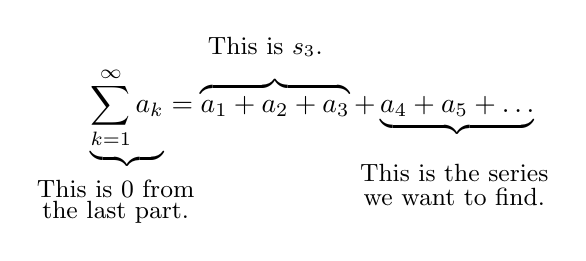
\begin{tikzpicture}
        \node at (0,0) {
          $\underbrace{\sum_{k=1}^{\infty} a_k}=\overbrace{a_1+a_2+a_3}+ \underbrace{a_4+a_5 + \ldots}$};
        \node at (1.8,-.7) {\small{This is the series}};
        \node at (1.8,-1) {\small{we want to find.}};
        
        \node at (-2.5,-.9) {\small{This is $0$ from }};
        \node at (-2.5,-1.2) {\small{the last part.}};    
        
        \node at (-.6,.9) {\small{This is $s_3$. }};
        
      \end{tikzpicture}
  \end{image}
  
 Putting this together, we have:
 
 \[
 0 = s_3 + \sum_{k=4}^{\infty} a_k,
 \] 
 and we find that $ \sum_{k=4}^{\infty} a_k = -1$. 

We can determine whether $\sum_{k=1}^{\infty} a_k$ converges or diverges by analyzing $\lim_{n \to \infty} s_n = \lim_{n \to \infty} \frac{8n^2}{n^4-9}$.  Since this limit is zero, we know that $\sum_{k=1}^{\infty} a_k$ converges to $0$.
\end{explanation}
\end{question}

\end{example}

\end{document}
